\documentclass[english]{article}
\renewcommand{\thesection}{\arabic{section}} % Redefine section numbering format
\usepackage[english]{babel} 
\usepackage[T1]{fontenc}
\usepackage[utf8x]{inputenc}
\usepackage{float}
\usepackage{graphicx}

\makeatletter
\usepackage[a4paper,top=2cm,bottom=2cm,left=2cm,right=2cm]{geometry}
\usepackage{enumitem}
\usepackage{subfig}
\usepackage{amsthm}
\usepackage{amsmath}
\usepackage{epstopdf}
\usepackage{fancyhdr}
\usepackage{booktabs,array}

\hyphenation{english}
\makeatother

\usepackage{babel}


\usepackage{listings}
\usepackage{xcolor} % for setting colors

% set the default code style
\lstset{
    frame=tb, % draw a frame at the top and bottom of the code block
    tabsize=4, % tab space width
    showstringspaces=false, % don't mark spaces in strings
    numbers=left, % display line numbers on the left
    commentstyle=\color{gray}, % comment color
    keywordstyle=\color{blue}, % keyword color
    stringstyle=\color{red} % string color
}

\begin{document}
\setcounter{section}{-1} % Set section counter to -1
\begin{titlepage}

	\begin{center}
		\begin{Large} \textbf{UNIVERSITY OF PADOVA} \\
		\end{Large} \vspace{1cm}
		\vspace{3cm}
		\begin{Large} Embedded Real--Time Control \end{Large}
		\par\end{center}

	\begin{center}
		\begin{Large}Laboratory report\\
		\end{Large}
		\par\end{center}

	\begin{center}
		\vspace{2cm}
		\begin{figure}[!htb]
			\centering 
\includegraphics[width=8cm]{figures/unipd-logo.png}\\

		\end{figure}

		\par\end{center}

	\begin{center}
		\vspace{2cm}
		\begin{Large} 
                Maximillime - (2096189) \\
                Mohammadjavad Rajabi - (2085121) \\
                Pouria Zakariapour - (2072836) \\
                Parsa Majidi - (2080216)  \\
		\end{Large} \vspace{2cm}
		\begin{Large} Academic Year 2022-2023 \end{Large}
		\par\end{center}

\end{titlepage}

\tableofcontents
\newpage
\section{Abstract}
During this course we worked with a turtlebot that you can see in the Figure \ref{fig:turtlebot}
The TurtleBot has several buttons, switches, and LEDs connected to the STM32F767 GPIOs
\begin{figure}[!h]
	\centering
	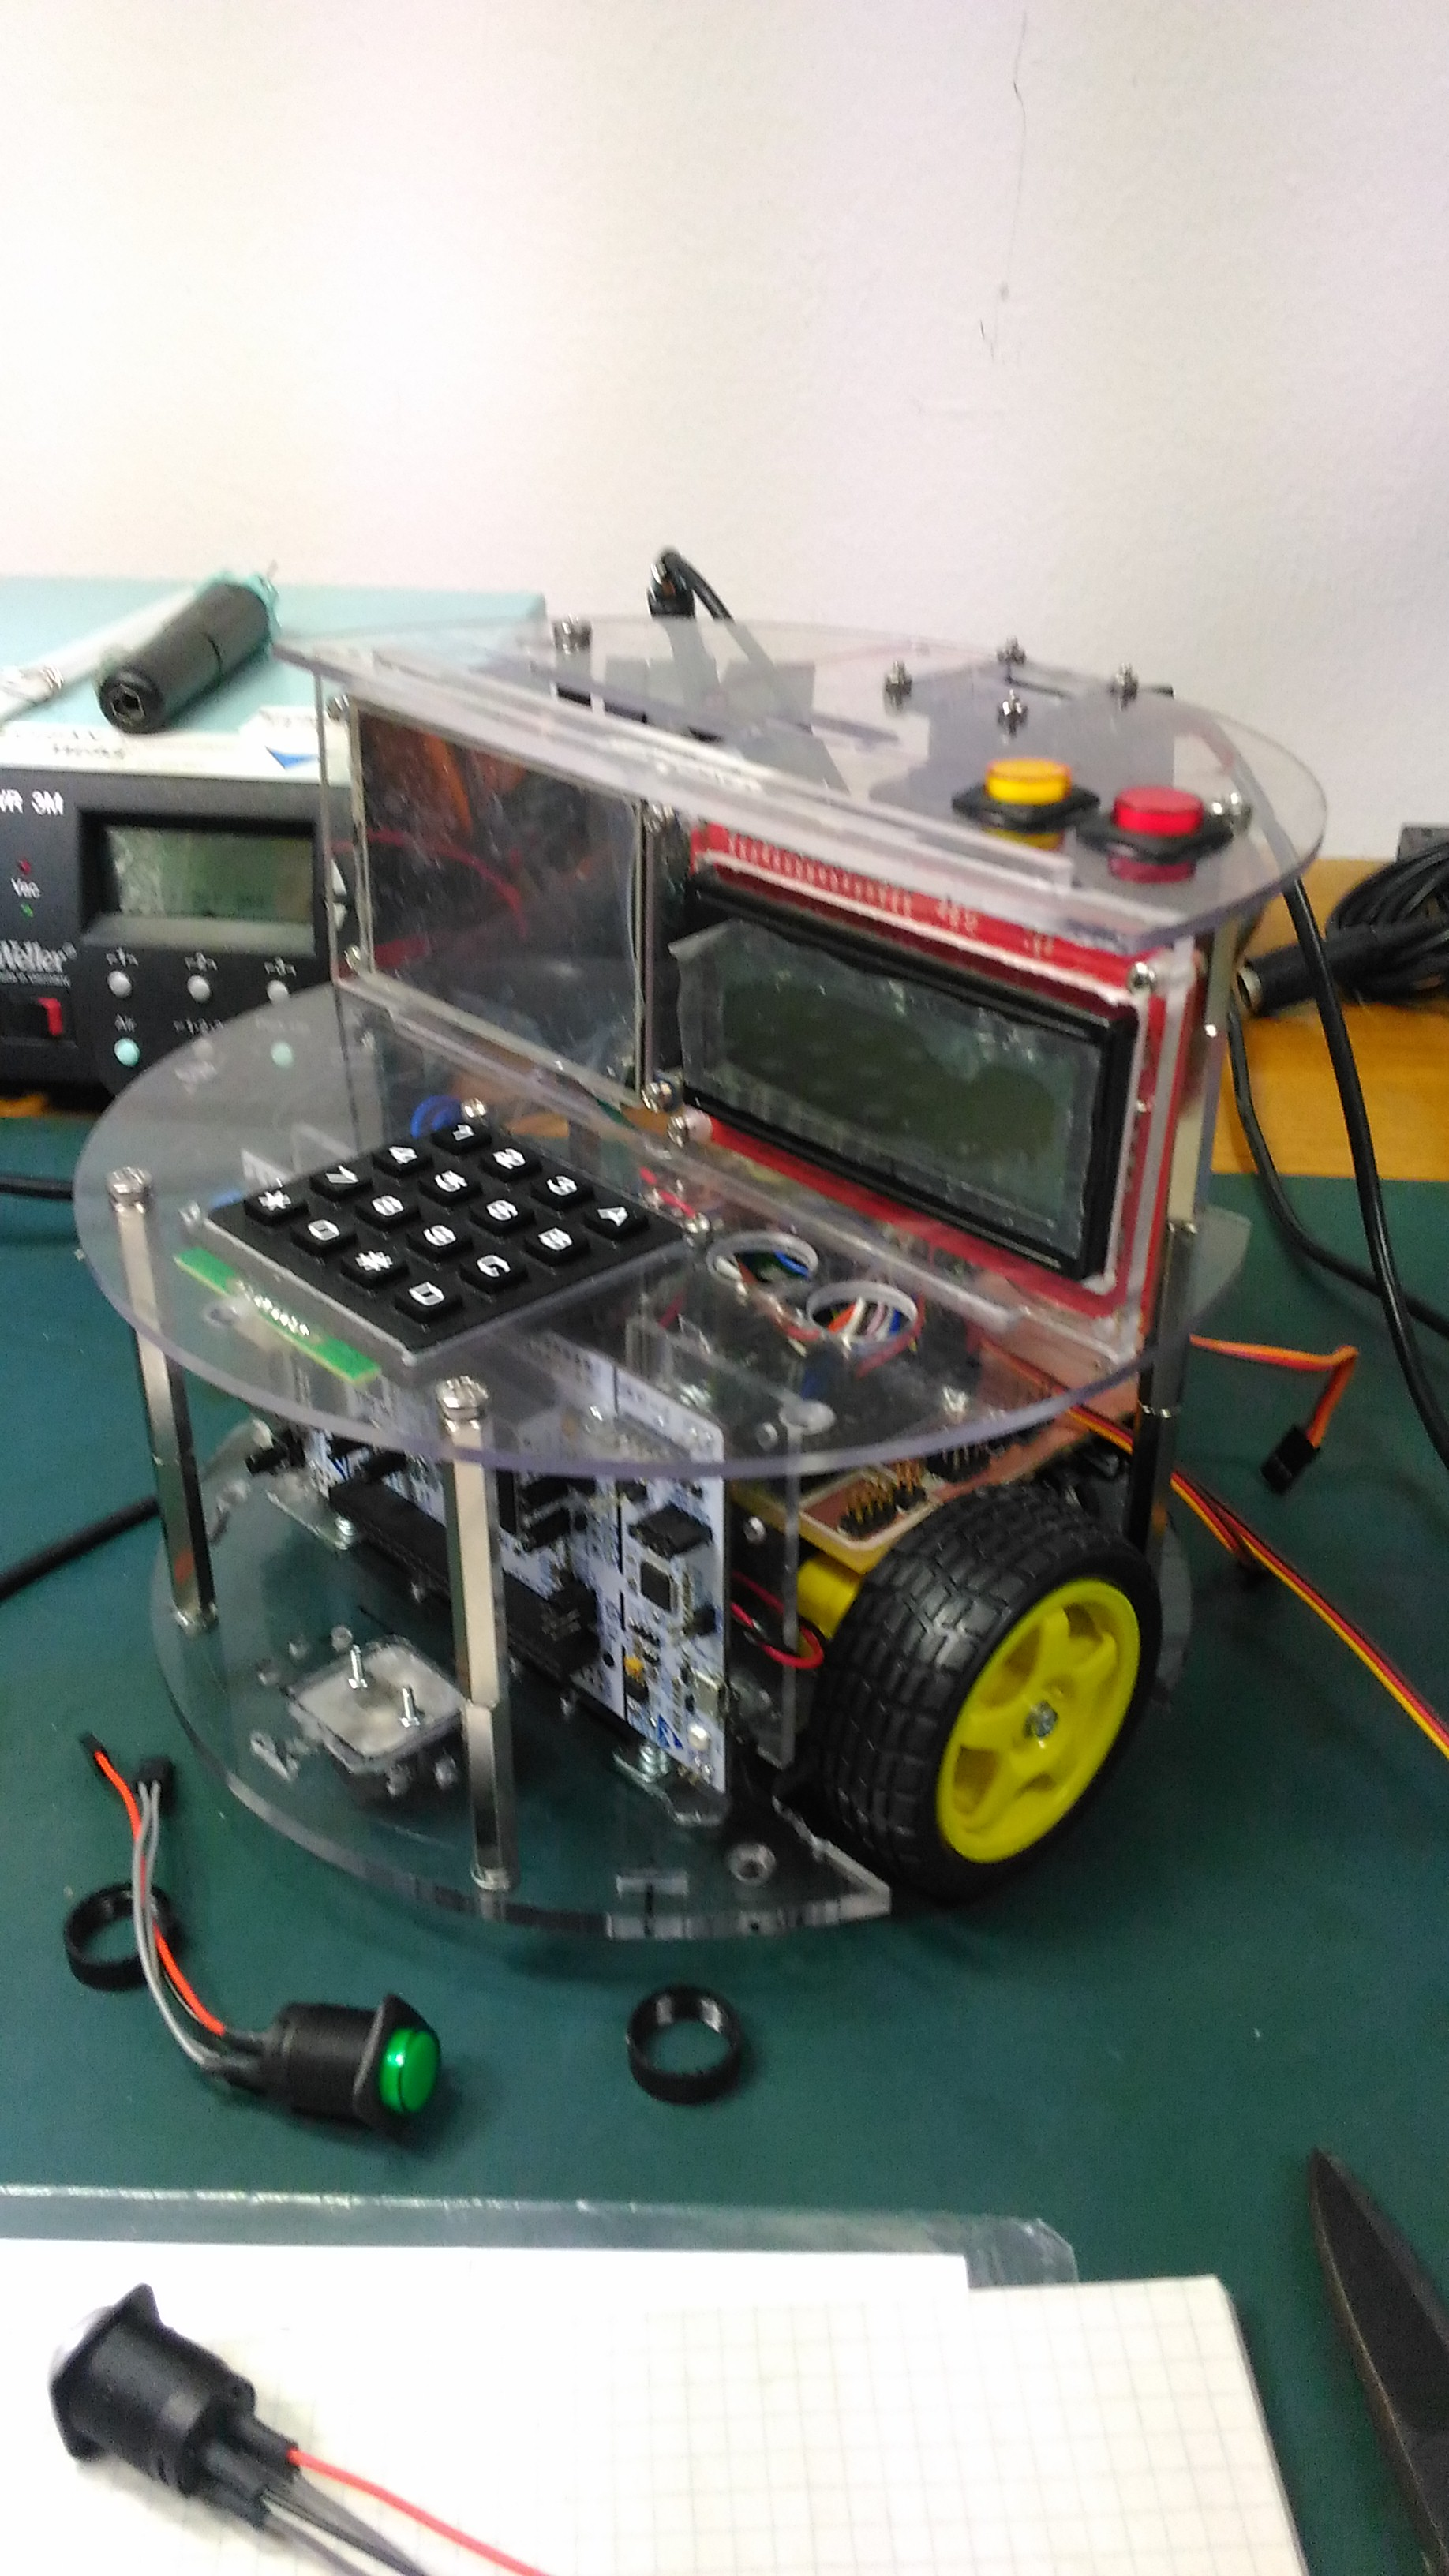
\includegraphics[width=0.4\textwidth]{figures/turtlebot_1.jpg}
	\caption{The TurtleBot}
	\label{fig:turtlebot}
\end{figure}

\newpage
\section{Laboratory 1: I2C}
The purpose of this lab can be categorized like below:
\begin{itemize}
    \item Inter-Integrated Circuit (I2C)
    \item SX1509 I/O Expander
    \item APIs
\end{itemize}

\subsection{Description}
This laboratory aims to explore and gain practical experience with some fundamental concepts in Embedded Systems.
 In particular, we will focus on working with the I2C protocol and the SX1509 module, as well as understanding 
and utilizing interrupts in the STM32F767 microcontroller. Throughout this laboratory, we will delve into several exercises that will provide us with hands-on experience in applying these concepts.

\subsection{Inter-Integrated Circuit (I2C)}
The I2C bus is a standard bidirectional interface that uses a controller, known as
the master, to communicate with slave devices, Shown in Figure \ref{fig:I2C}. 
\begin{figure}[!h]
	\centering
	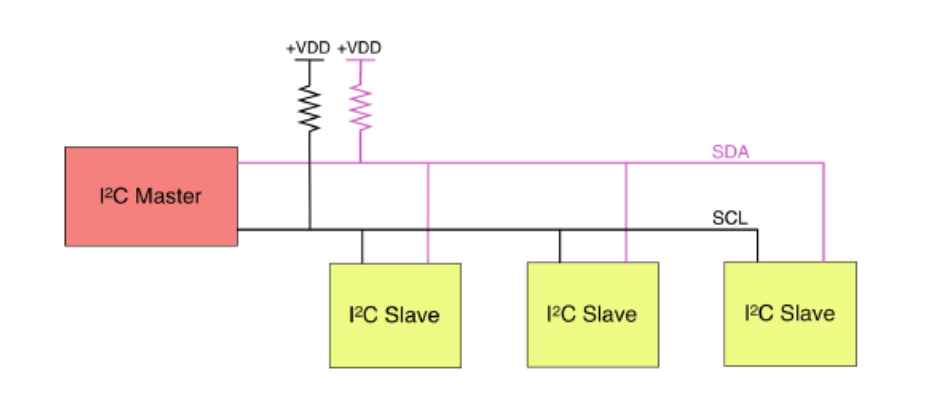
\includegraphics[width=0.65\textwidth,]{figures/I2C_Connection.png}
	\caption{I2C Connection Scheme}
	\label{fig:I2C}
\end{figure}

A slave may not transmit data unless it has been addressed by the master. 
Each device on the I2C bus has a specific device address to differentiate between
other devices that are on the same I2C bus. Many slave devices will require configuration upon startup to set the behavior of
the device. This is typically done when the master accesses the slave's internal
register maps, which have unique register addresses. A device can have one or
multiple registers where data is stored, written, or read. Many slave devices will require configuration upon startup to set the behavior of
the device. The physical I2C interface consists of the serial clock (SCL) and serial data (SDA) lines. 
Both SDA and SCL lines must be connected to VCC through a pull-up resistor. The size
of the pull-up resistor is determined by the amount of capacitance on the I2C lines.
Shown in Figure (\ref{fig:pulling}) and Figure (\ref{fig:releasing})
\begin{figure}[!ht]
	\centering
	\subfloat[Pulling the Bus Low with an open-drain Interface ]
	{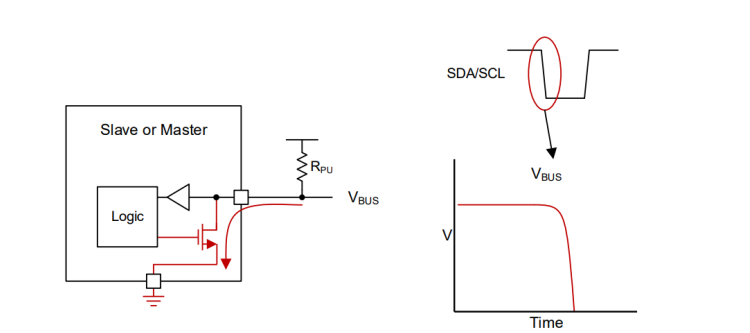
\includegraphics[width=0.45\textwidth,height=0.25\textwidth]{figures/Pulling-the-bus.png}
		\label{fig:pulling}}
	\subfloat[Releasing the bus with an open-drain interface]
	{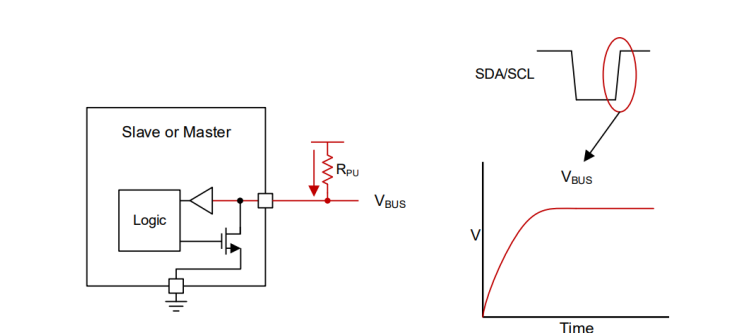
\includegraphics[width=0.45\textwidth,height=0.25\textwidth]{figures/Releasing-the-bus.png}
		\label{fig:releasing}}
	\caption{}
\end{figure}
\newpage
The protocol transmits messages composed by a 9 bit packet. Each message begins with
 the µC generation of a start signal and ends with a stop signal from the microcontroller,
 Shown in Figure \ref{fig:Stop}.
 \begin{figure}[!h]
	\centering
	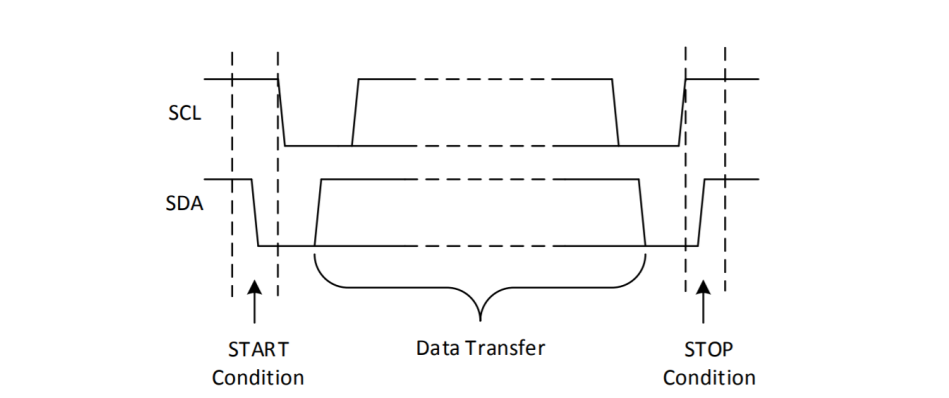
\includegraphics[width=0.80\textwidth,]{figures/Start-Stop.png}
	\caption{Example of Start and Stop condition}
	\label{fig:Stop}
\end{figure}
The start and stop conditions are characterized by data line that
moves towards low (start) or high (stop) during the clock high phase.
Any other bit is set during the low clock phase; this ensure that the
start and stop condition can be discriminated from any other data
transmission.\newline

In this communication protocol, each packet consists of 9 bits. 
The first 8 bits are transmitted by the sending unit, while the 9th bit is set by the receiving unit. 
The order of the bits within each byte follows a "Most Significant Bit" (MSB) format. 
The 9th bit serves as an acknowledgment, indicating whether the receiver acknowledges the data. 
To acknowledge, the receiver sets the data line to a low state at the 9th bit position.
Example of Single Byte data transfer in Figure \ref{fig:Data}.
\begin{figure}[!h]
	\centering
	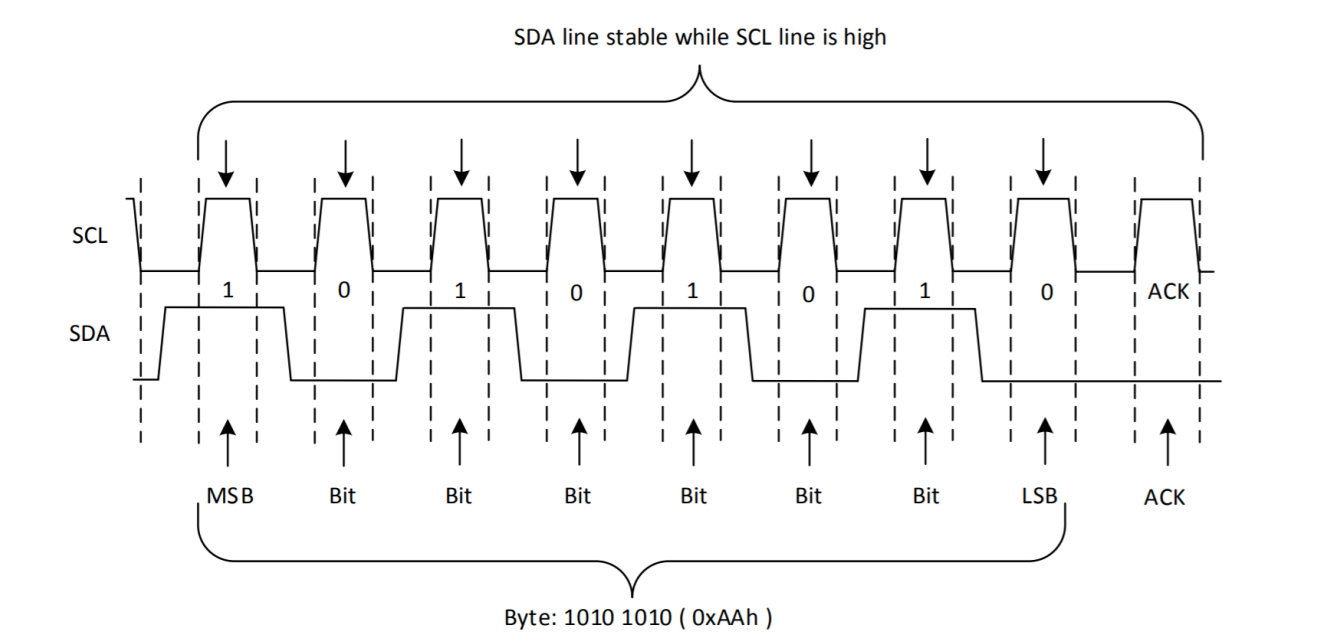
\includegraphics[width=0.80\textwidth,]{figures/Single_byte.png}
	\caption{Example of Single Byte Data Transfer}
	\label{fig:Data}
\end{figure}

\subsection{SX1509 I/O Expander}
The SX1509 is complete ultra
low voltage 1.2V to 3.6V General Purpose parallel
Input/Output (GPIO) expanders ideal for low power
handheld battery powered equipment. This family of
GPIOs comes in 4-, 8-, 16-channel configuration and
allows easy serial expansion of I/O through a
standard 400kHz I2C interface. GPIO devices can
provide additional control and monitoring when the
microcontroller or chipset has insufficient I/O ports, or
in systems where serial communication and control
from a remote location is advantageous. Keypad application is also supported with
the on-chip scanning engine which enables
continuous keypad monitoring up to 64 keys without
any additional host interaction and further reduce the
bus activity. The SX1509 has the ability to
generate mask-programmable interrupts based on
falling/rising edge of any of its GPIO lines. \newline

In this setup, two SX1509 modules are connected to the microcontroller using the I2C bus. 
Both devices share the same I2C line, specifically I2C1. To differentiate between the two modules,
we assign a specific slave address to each. 
The first SX1509, referred to as sx1509\_1, is assigned
  the slave address 0x3E, while the second module, known as sx1509\_2, is associated with the slave address 0x3F.
\\Allocated addresses of slaves implemented in Code \ref{lst:addr}
\begin{lstlisting}[language=C, caption={I2C Addresses}, label={lst:addr} ]
#define SX1509_I2C_ADDR1 0x3E       //SX1509 Proxy Sensors I2C address
#define SX1509_I2C_ADDR2 0x3F       //SX1509 Keypad I2C address
\end{lstlisting}
The two lines of Code \ref{lst:add} are addressing of SX1509 registes for Keypad.
\begin{lstlisting}[language=C, caption={Keypad Data registers}, label={lst:add} ]
#define REG_KEY_DATA_1  0x27        //RegKeyData1 Key value (column) 1111 1111
#define REG_KEY_DATA_2  0x28	    //RegKeyData2 Key value (row) 1111 1111
\end{lstlisting}
This addressing scheme allows the microcontroller to communicate with each SX1509 module individually over the shared I2C bus.
Figure \ref{fig:SX1509}
\begin{figure}[!h]
	\centering
	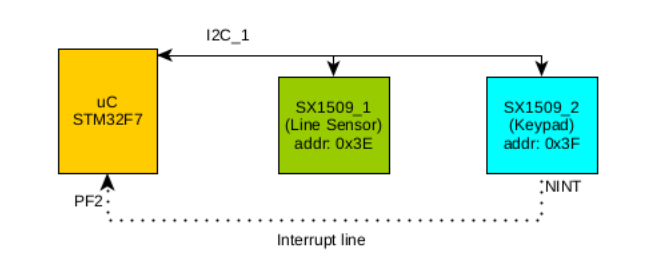
\includegraphics[width=0.80\textwidth,]{figures/SX.png}
	\caption{SX1509 connected to Keypad and Line sensor}
	\label{fig:SX1509}
\end{figure}
\subsection{APIs}
The HAL (Hardware Abstraction Layer) API (Application Programming Interface) 
is a software layer provided by STM32 microcontrollers that abstracts
 the underlying hardware functionalities and provides a standardized 
 interface for developers to interact with the microcontroller's peripherals and features.
The HAL API serves as a bridge between the application software and the hardware, 
allowing developers to access and control the microcontroller's peripherals,
such as GPIO (General Purpose Input/Output), UART (Universal Asynchronous Receiver-Transmitter),
SPI (Serial Peripheral Interface), I2C (Inter-Integrated Circuit), 
timers, and more. It provides a higher-level programming interface,
hiding the low-level hardware details and offering a set of functions that
encapsulate complex hardware operations. \newline
Following are useful HAL functions that we used during this Laboratory.
\begin{lstlisting}[language=C, caption={Reading Register values}, label={lst:read} ]
HAL_StatusTypeDef HAL_I2C_Mem_Read(I2C_HandleTypeDef *hi2c, uint16_t
    DevAddress, uint16_t MemAddress, uint16_t MemAddSize, uint8_t *pData,
    uint16_t Size, uint32_t Timeout);
\end{lstlisting}
Read an amount of data in blocking mode from a specific memory address  
\begin{itemize}
    \item \textbf{hi2c} Pointer to a I2C\_HandleTypeDef structure that contains the configuration information
    for the specified I2C.
    \item \textbf{DevAddress} Target device address: The device 7 bits address value in datasheet must be
    shifted to the left before calling the interface.
    \item \textbf{MemAddress} Internal memory address
    \item \textbf{MemAddSize} Size of internal memory address
    \item \textbf{pData} Pointer to data buffer
    \item \textbf{Size} Amount of data to be sent
    \item \textbf{Timeout} Timeout duration
    \item \textbf{return value} HAL status
\end{itemize}

\begin{lstlisting}[language=C, caption={Writing Register values}, label={lst:write} ]
HAL_StatusTypeDef HAL_I2C_Mem_Write(I2C_HandleTypeDef *hi2c, uint16_t
    DevAddress, uint16_t MemAddress, uint16_t MemAddSize, uint8_t *pData,
    uint16_t Size, uint32_t Timeout)
\end{lstlisting}
Write an amount of data in blocking mode to a specific memory address
\begin{itemize}
    \item \textbf{hi2c} Pointer to a I2C\_HandleTypeDef structure that contains the configuration information
        for the specified I2C.
        \item \textbf{DevAddress} Target device address: The device 7 bits address value in datasheet must be
        shifted to the left before calling the interface.
        \item \textbf{MemAddress} Internal memory address
        \item \textbf{MemAddSize} Size of internal memory address
        \item \textbf{pData} Pointer to data buffer
        \item \textbf{Size} Amount of data to be sent
        \item \textbf{Timeout} Timeout duration 
        \item \textbf{return value} HAL status
\end{itemize}

\newpage
\subsection{Exercise 1:}
\subsubsection{Description}
In this exercise we are asked to write an ISR that recognize and correctly handles the keypad interrupts. We properly implemented the void HAL\_GPIO\_EXTI\_Callback(uint16\_t pin) function, which is used in conjunction with the EXTI (External Interrupt) peripheral to handle interrupts generated by GPIO pins. Then we printed which interrupt has
been triggered i.e. the pin. To be able to receive another interrupt from the keypad, we read
the registers REG\_KEY\_DATA\_1 and REG\_KEY\_DATA\_2 inside the ISR.
\subsubsection{Code}
\begin{lstlisting}[language=C, caption={Interrupt Callback}]
void HAL_GPIO_EXTI_Callback(uint16_t GPIO_Pin){
    /*Reading Data From SX1509_I2C_ADDR2 Device Address and REG_KEY_DATA_1 and 
    REG_KEY_DATA_2 Memory Addresses */
    HAL_StatusTypeDef status;
    status = HAL_I2C_Mem_Read(
        &hi2c1,
        SX1509_I2C_ADDR2 << 1,
        REG_KEY_DATA_1,
        1,
        &colum,
        1,
        I2C_TIMEOUT
    );
    if (status != HAL_OK) {
        printf("Error occurred during reading I2C, REG_KEY_DATA_1\n");
    }
    status = HAL_I2C_Mem_Read(
        &hi2c1,
        SX1509_I2C_ADDR2 << 1,
        REG_KEY_DATA_2, 1,&row,
        1, 
        I2C_TIMEOUT
    );
    if (status != HAL_OK) {
        printf("Error occurred during reading I2C, REG_KEY_DATA_2\n");
    }
    printf("Interrupt on pin (%d).\n", GPIO_Pin);
}
\end{lstlisting}

\subsubsection{Code Explanation:}
in this code we have implemented callback interrupt ...
%See code~\ref{lst:label}.
\newpage
\subsection{Exercise 2:}
\subsubsection{Description:}
In this exercise we had to extend the code of exercise 1 to handle the keypad interrupt. we printed which keypad button has been pressed.
\subsubsection{Code:}
\begin{lstlisting}[language=C, caption={Pressed Keypad Button}, label={lst:label} ]
const char keypadLayout[4][4] = {
    {'*', '0', '#', 'D'},
    {'7', '8', '9', 'C'},
    {'4', '5', '6', 'B'},
    {'1', '2', '3', 'A'}
};
int colum, row;
char triggeredChar;
int columDir [4]= { 3, 2 ,1 ,0};
int getIndex(int value);

void HAL_GPIO_EXTI_Callback(uint16_t GPIO_Pin){

    HAL_StatusTypeDef status;
    status = HAL_I2C_Mem_Read(
        &hi2c1,
        SX1509_I2C_ADDR2 << 1,
        REG_KEY_DATA_1,
        1,
        &colum,
        1,
        I2C_TIMEOUT
    );
    if (status != HAL_OK) {
        printf("Error occurred during reading I2C, REG_KEY_DATA_1\n");
    }
    status = HAL_I2C_Mem_Read(
        &hi2c1,
        SX1509_I2C_ADDR2 << 1,
        REG_KEY_DATA_2, 1,&row,
        1, 
        I2C_TIMEOUT
    );
    if (status != HAL_OK) {
        printf("Error occurred during reading I2C, REG_KEY_DATA_2\n");
    }
    printf("Interrupt on pin (%d).\n", GPIO_Pin);
    printf("colum.raw (%d)    row.raw (%d).\n", colum, row);
    colum = getIndex (colum);
    row = getIndex(row);
    printf("colum (%d)    row (%d).\n", colum, row);
    triggeredChar = keypadLayout[row][colum];
} //End of Interrupt Callback function
int getIndex(int value){
  switch (value){
    case 247:
      return 3;
    case 251:
      return 2;
    case 253:
      return 1;
    case 254:
      return 0;
    default:
      return 99;
  }
}
\end{lstlisting}

\subsubsection{Code Explanation:}
%See code~\ref{lst:label}.
\newpage
\subsection{Exercise 3:}
\subsubsection{Description:}
In this exercise we had to write a routine that reads the status of the line sensor and prints it. The routine must check the status with a polling period of 100ms.
\subsubsection{Code:}
\begin{lstlisting}[language=C, caption={Reading Line Data}, label={lst:label} ]
int findBinary(int decimal){
	int base = 1;
	int binary = 0;
   while(decimal > 0){
	   int rem = decimal % 2;
	   binary = binary + rem*base;
	   decimal = decimal / 2;
	   base = base * 10;
   }
   printf("Binary: %d\n\r", binary);
}//End of findBinary Function
int lineData;
while (1){
    HAL_I2C_Mem_Read(
        &hi2c1,
        SX1509_I2C_ADDR1 << 1,
        REG_DATA_B,
        1,
        &lineData,
        1,
        I2C_TIMEOUT
        );
	  findBinary(lineData);
	  printf("Decimal is: %d \n\r", lineData);
	  HAL_Delay(100);
}//End of While loop
\end{lstlisting}
\subsubsection{Code Explanation:}
sadklasjdlkasjdl
%See code~\ref{lst:label}.

\newpage
\subsection{Exercise 4:}
\subsubsection{Description:}
We made one LED blinking. If you use LEDs connected to PE5 or PE6, check the *.ioc to make sure that those pins are set as GPIO\_output. The blinking frequency should be
set by the user through the keypad. There’s two way to do this:
Hard way (Bonus): The frequency can be set “dynamically” by the user. For example, if the user
press 125\# the LED should blink with a frequency of 125Hz. If the user press 250\# the LED should
blink with a frequency of 250Hz, and so on.
\subsubsection{Code:}
\begin{lstlisting}[language=C, caption={C code using listings}, label={lst:label} ]
//These are Global Variables//
int inputUser = 0;
int counter = 0;
int flag=0;
int freq;

//This part of code has implemented in the Interrupt Callback Function
triggeredChar = keypadLayout[row][colum];
if(flag == 1){
    freq = inputUser;
    inputUser = 0;
    counter = 0;
    flag = 0;
}
if((triggeredChar <= '9') && (triggeredChar >= '0')){
    keypadFreq = (int)(triggeredChar - '0');
    inputUser = inputUser*(10^counter) + keypadFreq;
    counter++;
}
  printf("Triggered Char: %c \n\r ", triggeredChar);
//End of Interrupt Callback function


//Start infinit loop
while (1){
    if(triggeredChar == '#'){
	flag = 1;
	HAL_GPIO_TogglePin(GPIOE, GPIO_PIN_5);
	   if(inputUser != 0){
		HAL_Delay((1.0/inputUser)*1000);
	   }
	   else{
		HAL_Delay(1000);
	   }
    }//End of if(triggerChar ..)
    else{
        HAL_GPIO_TogglePin(GPIOE, GPIO_PIN_5);
        if(freq != 0){
        HAL_Delay((1.0/freq)*1000);
        }
        else{
            HAL_Delay(1000);
        }
    }
}//End of While loop
\end{lstlisting}
\subsubsection{Code Explanation:}
%See code~\ref{lst:label}.
\newpage
\section{Laboratory 2: Open loop control (camera stabilizer)}
In this lab we are going to implement an open loop stabilizer
using the IMU and servo motors.
\subsection{IMU}
IMU stands for Inertial Measurement Unit. It is a device that is used 
to measure and report an object's specific force, angular rate, and 
sometimes the magnetic field surrounding it. IMUs are commonly used in
 various applications, including robotics, navigation systems, virtual 
 reality, augmented reality, and motion capture.\newline

An IMU typically consists of several sensors that work together to
provide information about an object's motion and orientation:
\begin{itemize}
    \item \textbf{Accelerometer}: Measures linear acceleration along different axes 
    (typically three axes: X, Y, and Z). It detects changes in velocity 
    and orientation, allowing the IMU to determine the object's 
    acceleration and tilt. Figure (\ref{fig:acc})
    \item \textbf{Gyroscope}: Measures angular velocity or rate of rotation 
    around different axes. It provides information about the object's 
    rotational motion and helps track changes in orientation.
    \item \textbf{Magnetometer}: Measures the strength and direction of the
     magnetic field around the object. It is often included in IMUs to 
     provide additional information for orientation estimation,
    especially when used in combination with accelerometers and
    gyroscopes. 
\end{itemize}
By combining the data from these sensors, an IMU can estimate the
 object's orientation, position, and velocity relative to its initial 
 state. 
 \begin{figure}[!h]
     \centering
     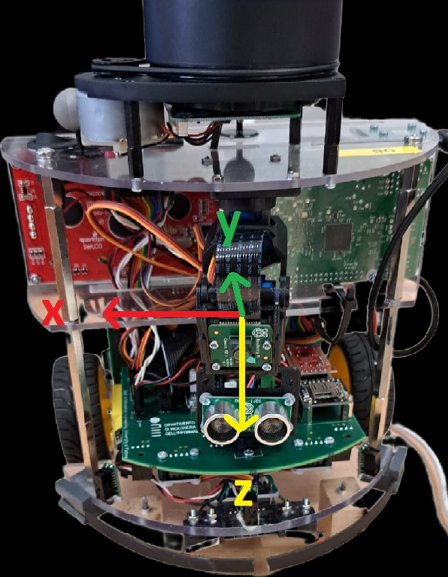
\includegraphics[width=0.50\textwidth, height=0.4\textheight]{figures/Lab2_1.png}
     \caption{The axis of the accelerometer}
     \label{fig:acc}
 \end{figure}
 \begin{itemize}
    \item \textbf{Tilt} refers to the vertical movement 
    of the camera, where the camera is moved up or down.
    \item \textbf{Pan} refers to the horizontal movement of the 
    camera, where the camera is rotated around its vertical axis
     to the left or right. 
 \end{itemize}
\subsection{Servo Motor}
A servo motor is a type of motor that is widely used in various 
applications, particularly in robotics, automation, and control systems.
It is designed to provide precise control over angular or rotational
movement. \newline

The distinguishing feature of a servo motor is its ability to maintain
 a specific position or follow a desired trajectory with great accuracy.
It achieves this through a closed-loop control system, which continuously
compares the actual position of the motor shaft with the desired position
and adjusts the motor's output accordingly. 

Here are some key components and characteristics of servo motors: 
\begin{itemize}
    \item \textbf{DC Motor}: Most servo motors are based on a DC motor
     as the primary driving mechanism. The DC motor converts electrical 
     energy into rotational motion. 
     \item \textbf{Gear Train}: Servo motors often include a gear train
      that reduces the motor's high-speed, low-torque output to a lower
       speed with higher torque. This gearing mechanism enables the servo
      motor to generate more precise and controlled movements.
    \item \textbf{Position Feedback Sensor}: A servo motor typically 
    incorporates a position feedback sensor, such as an encoder or a
     potentiometer. This sensor provides information about the current 
     position and velocity of the motor shaft. The feedback data is used
      by the control system to determine if the motor needs to adjust its 
    position.
    \item \textbf{Control Circuitry}: The control circuitry of a servo motor
     includes a microcontroller or a dedicated servo controller.
      It receives the control signal or command from an external device,
       such as a microcontroller or a computer, and generates the appropriate
        electrical signals to drive the motor. 
    \item \textbf{Pulse Width Modulation (PWM) Signal}: Servo motors commonly 
    utilize a PWM signal to control their position and speed. The control signal
     consists of a series of pulses with varying widths, where the width of each 
     pulse determines the desired position. The control circuitry interprets the
      pulse width and adjusts the motor's position accordingly. Figure (\ref{fig:PWM})
\end{itemize}
\begin{figure}[!h]
    \centering
    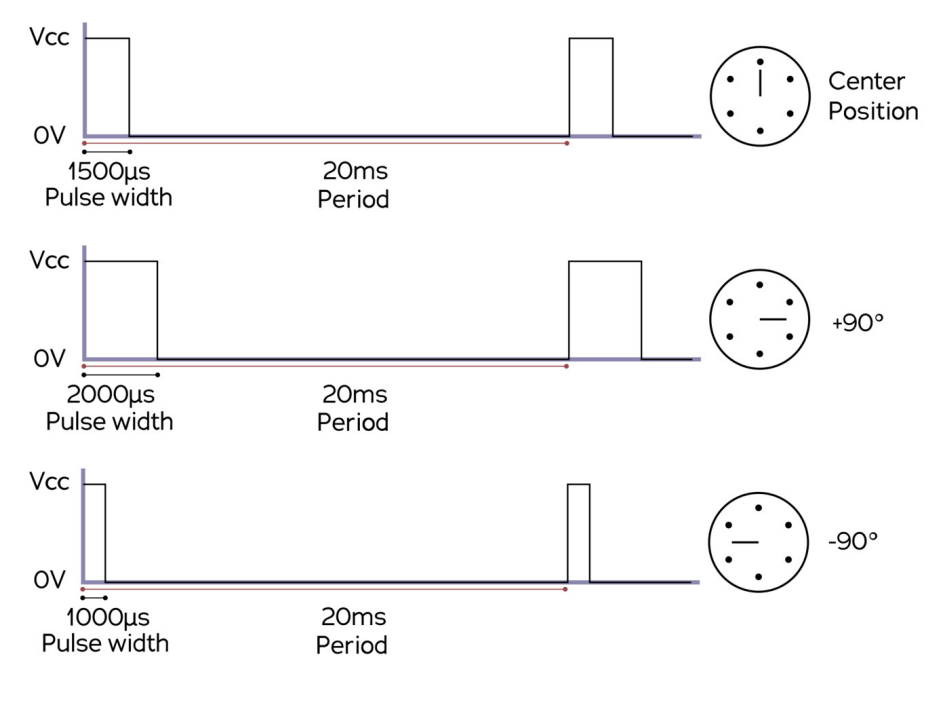
\includegraphics[width=0.80\textwidth, height=0.35\textheight]{figures/PWM.png}
    \caption{PWM signal and comtroling the position of the motor}
    \label{fig:PWM}
\end{figure}
\newpage
On the TurtleBot these are two servo that control the tilt and pan of a camera
as shown in the figure below. Figure (\ref{fig:motor})
\begin{figure}[!h]
    \centering
    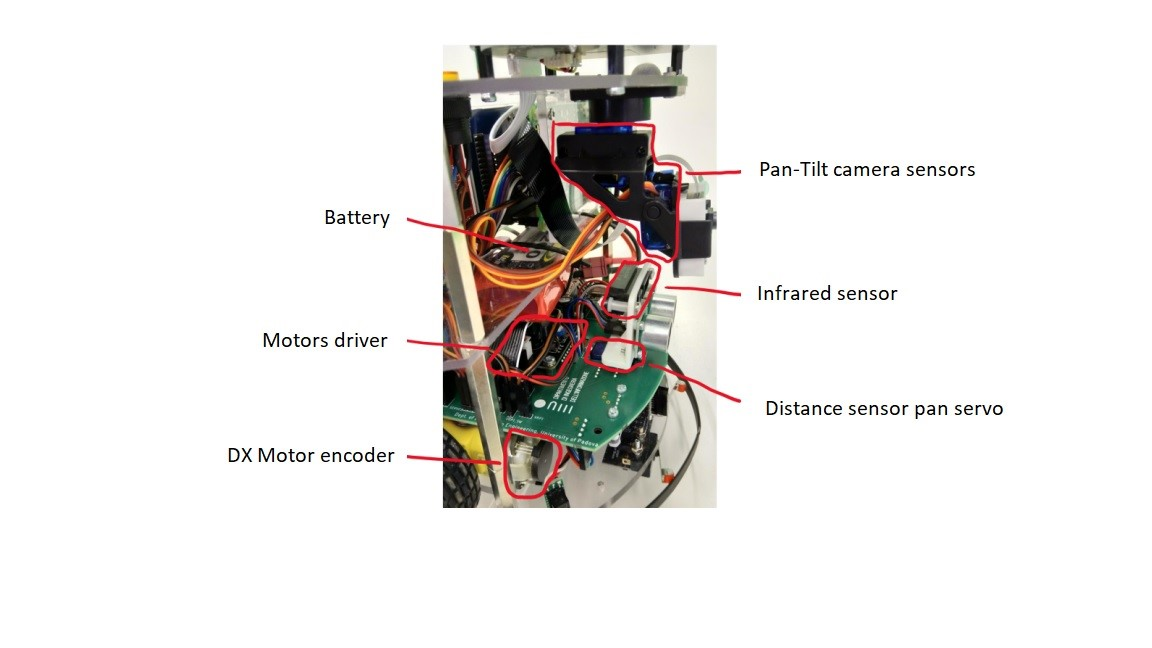
\includegraphics[width=1.10\textwidth, height=0.35\textheight]{figures/motor.png}
    \caption{PWM signal and comtroling the position of the motor}
    \label{fig:motor}
\end{figure}
\subsection{Exercise1:}
Develop a control law to stabilize the camera’s tilt by utilizing data from an IMU. \newline
First of all, we have to keep the camera aligned (0 degree) with the horizon. For
this purpose, we should obtain the accelerometer and gyroscope data from the robot.
\begin{lstlisting}[language=C, caption={C code using listings}, label={lst:label} ]

    int8_t tilt = 0; 
    float angle = 0; 
while (1) { 

    HAL_Delay(20); 
    bno055_convert_double_accel_xyz_msq(&d_accel_xyz); 
    angle = (asin(d_accel_xyz.y/ 9.81)) * 180 / 3.14; 
    tilt = -angle; 
    logger_data.u1 = tilt; 
    logger_data.u2 = d_accel_xyz.y; 
    ertc_dlog_send(&logger, &logger_data, sizeof(logger_data)); 
    ertc_dlog_update(&logger); 

    __HAL_TIM_SET_COMPARE(&htim1,
        TIM_CHANNEL_3,
        (uint32_t)saturate((150+tilt*(50.0/5.0)),
         SERVO_MIN_VALUE, 
         SERVO_MAX_VALUE));  

   } 
\end{lstlisting}
As you see, first we defined tilt and angle globally. 
To obtain the accelerometer data we use “bno055\_convert\_double
\_accel\_xyz\_msq”
and “d\_accel\_xyz” as a pointer to a structure as input.
\newpage
The formula for finding the tilt of Tbot is: 
\textbf{$\theta = \sin^{-1}\left(\frac{a_y}{g}\right)$} which $\theta$ is the tilt angle,
${a_y}$ is the acceleration measured on the y axis and g is gravity acceleration (=9.81).
To convert $\theta$ from radiant the equation should be multiplied by ($\frac{180}{\pi}$)
As we want to put the camera aligned we should put the tilt equal to (-$\theta$) 
otherwise the camera turns reverse. \newline
For moving the camera we use “\_\_HAL\_TIM\_SET\_COMPARE” Which is a HAL library macro
 used for setting the compare value of a specific channel of a hardware timer on a
  microcontroller. \newline

  To record the data, we use datalogger. As all the configuration for using the 
  datalogger is already done, first we define a structure to send the data:
\begin{lstlisting}[language=C, caption={}, label={lst:datalog} ]
struct ertc_dlog logger; 

struct datalog { 
    float u1, u2; 
} logger_data;  
\end{lstlisting} 

Then we use logger\_data.u1 as the tilt data and logger\_data.u2 as the acceleration
measured on the y axis data in the while loop. 
\newline

To plot the\ data we use Matlab and the serial datalogger is invoked using serial\_datalog()
 function as below: 
\begin{lstlisting}[language=Matlab, caption={}, label={lst:datalog} ]
data = serial_datalog('COM9',{'2*single','2*single'}, 'baudrate', 115200)
\end{lstlisting}
“COM9” is the port of the serial datalogger. “single,single” specifies the data 
format to be logged. It indicates that two data values will be logged in each 
iteration of the logging process. In this case, the logged data is expected to be
of type single (a single-precision floating-point number).\newline  
“baudrate”, “115200” sets the baud rate of the serial communication. 
The baud rate determines the speed at which data is transferred over the serial port.
 In this case, the baud rate is set to 115200 bits per second. 
 \begin{figure}[!h]
    \centering
    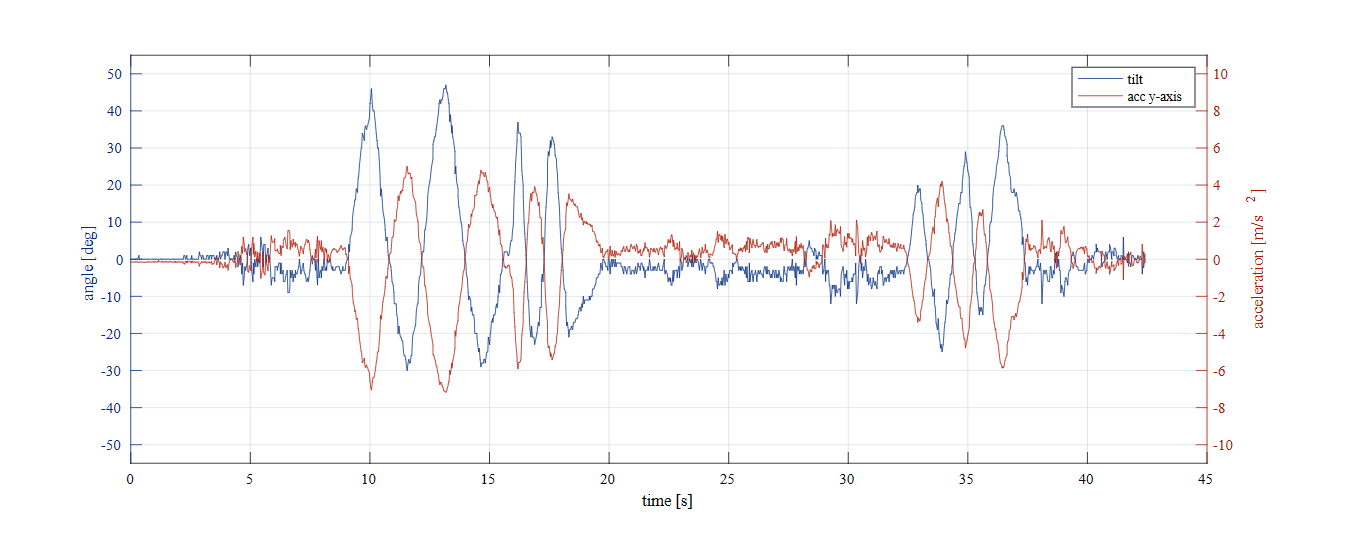
\includegraphics[width=1.0\textwidth, height=0.35\textheight]{figures/plot.png}
    \caption{Datalogger Plot}
    \label{fig:datal}
\end{figure}
\subsection{Bonus:}
Implement a control algorithm that implement a “smooth pan” control
(i.e. a control system that compensate sharp horizontal rotations of the TBot) 
using data from the gyroscope.\newline
Process is like exercise 1:
\newpage
\begin{lstlisting}[language=C, caption={}, label={lst:datalog} ]
    int8_t pan = 0; 

    float angle = 0; 
while (1) { 
    HAL_Delay(20); 
    bno055_convert_double_gyro_xyz_rps(&d_gyro_xyz);
    angle = d_gyro_xyz.z * 180 / 3.14;
    pan = -angle/8;
    logger_data.u1 = pan; 
    logger_data.u2 = d_gyro_xyz.z; 
    ertc_dlog_send(&logger, &logger_data, sizeof(logger_data)); 
    ertc_dlog_update(&logger); 
    __HAL_TIM_SET_COMPARE(&htim1,TIM_CHANNEL_3,
    (uint32_t)saturate((150+pan*(50.0/55.0)),
     SERVO_MIN_VALUE,
    SERVO_MAX_VALUE));   
} 
\end{lstlisting}
As it is clear to obtain the $\theta$ we have to put the gyroscope data measured in z axis and we put the pan equal to
(-$\frac{\theta}{8}$) which the negative sign is because of turning up and down
 properly and is divided to 8 which is the proper gain, and inside the “\_\_HAL\_TIM\_SET\_COMPARE()”, as the channel 3 is controlling the pan, 
 we should put “TIM\_CHANNEL\_3” instead of “TIM\_CHANNEL\_2” which is controlling the tilt. 
 \begin{figure}[!h]
    \centering
    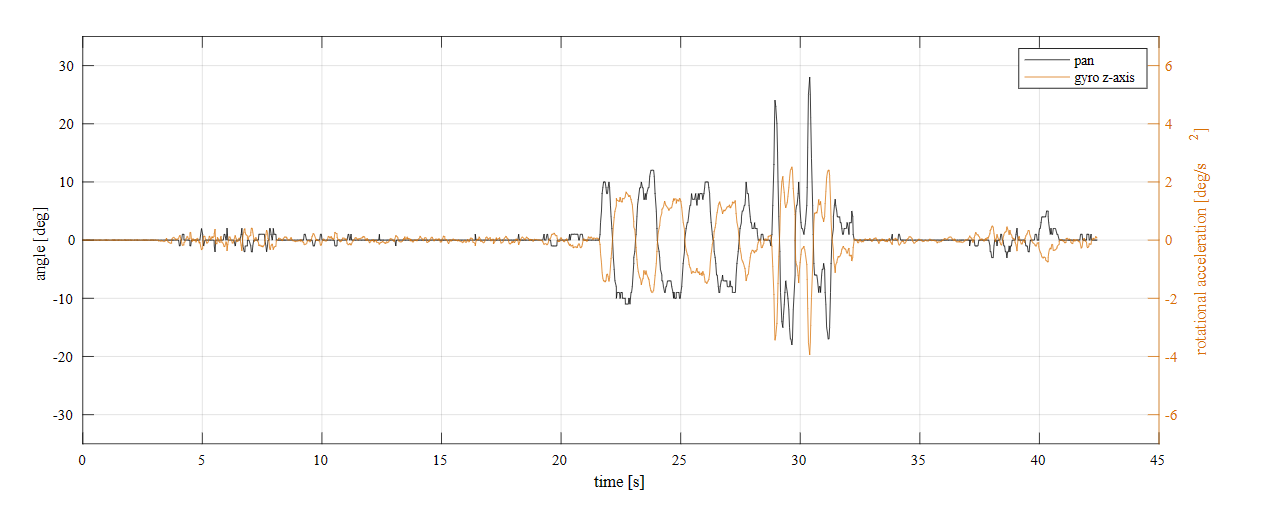
\includegraphics[width=1.0\textwidth, height=0.35\textheight]{figures/plot2.png}
    \caption{Datalogger Plot2}
    \label{fig:datal2}
\end{figure}
\newpage
\section{Laboratory 3: Motor Control}

\subsection{Relevant theoretical notions}

\subsection{Another sub}

\subsection{Another sub}

\newpage
\section{Laboratory 4: Line Following}

\subsection{Relevant theoretical notions}

\subsection{Another sub}

\subsection{Another sub}

\clearpage
\appendix

\section{Section in the Appendix}
\label{sec:app1}

\subsection{Subsection in the Appendix}
\label{subsec:app2}

Additional relevant information...

\end{document}
